\documentclass[12pt,letterpaper]{article}
\usepackage{graphicx,textcomp}
\usepackage[T1]{fontenc}
\usepackage{natbib}
\usepackage{setspace}
\usepackage{fullpage}
\usepackage{color}
\usepackage[reqno]{amsmath}
\usepackage{amsthm}
\usepackage{fancyvrb}
\usepackage{amssymb,enumerate}
\usepackage[all]{xy}
\usepackage{endnotes}
\usepackage{lscape}
\newtheorem{com}{Comment}
\usepackage{float}
\usepackage{hyperref}
\newtheorem{lem} {Lemma}
\newtheorem{prop}{Proposition}
\newtheorem{thm}{Theorem}
\newtheorem{defn}{Definition}
\newtheorem{cor}{Corollary}
\newtheorem{obs}{Observation}
\usepackage[compact]{titlesec}
\usepackage{dcolumn}
\usepackage{tikz}
\usetikzlibrary{arrows}
\usepackage{multirow}
\usepackage{xcolor}
\newcolumntype{.}{D{.}{.}{-1}}
\newcolumntype{d}[1]{D{.}{.}{#1}}
\definecolor{light-gray}{gray}{0.65}
\usepackage{url}
\usepackage{listings}
\usepackage{color}

\definecolor{codegreen}{rgb}{0,0.6,0}
\definecolor{codegray}{rgb}{0.5,0.5,0.5}
\definecolor{codepurple}{rgb}{0.58,0,0.82}
\definecolor{backcolour}{rgb}{0.95,0.95,0.92}

\lstdefinestyle{mystyle}{
	backgroundcolor=\color{backcolour},   
	commentstyle=\color{codegreen},
	keywordstyle=\color{magenta},
	numberstyle=\tiny\color{codegray},
	stringstyle=\color{codepurple},
	basicstyle=\footnotesize,
	breakatwhitespace=false,         
	breaklines=true,                 
	captionpos=b,                    
	keepspaces=true,                 
	numbers=left,                    
	numbersep=5pt,                  
	showspaces=false,                
	showstringspaces=false,
	showtabs=false,                  
	tabsize=2
}
\lstset{style=mystyle}
\newcommand{\Sref}[1]{Section~\ref{#1}}
\newtheorem{hyp}{Hypothesis}

\title{Problem Set 1}
\date{Due: January 27, 2020}
\author{QTM 200: Applied Regression Analysis}

\begin{document}
	\maketitle
	
	\section*{Instructions}
	\begin{itemize}
		\item Please show your work! You may lose points by simply writing in the answer. If the problem requires you to execute commands in \texttt{R}, please include the code you used to get your answers. Please also include the \texttt{.R} file that contains your code. If you are not sure if work needs to be shown for a particular problem, please ask.
		\item Your homework should be submitted electronically on the course GitHub page in \texttt{.pdf} form.
		\item This problem set is due at the beginning of class on Wednesday, January 22, 2020. No late assignments will be accepted.
		\item Total available points for this homework is 100.
	\end{itemize}
	
	\vspace{1cm}
	\section*{Question 1 (25 points)}

A private school counselor was curious about the average of IQ of the students in her school and took a random sample of 25 students' IQ scores. The following is the data set:
\vspace{.5cm}

\lstinputlisting[language=R, firstline=40, lastline=40]{PS1.R}  

\vspace{.5cm}

\noindent Find a 90\% confidence interval for the student IQ in the school assuming the population of IQ from which our random sample has been selected is normally distributed. 

\newpage

\noindent \textbf{\section*{Answer:}}

\noindent First, I calculated the t-score for a t-distribution with 24 degrees of freedom (degrees of freedom = sample size - 1; 25 - 1 = 24) using the qt function.  I used the t-distribution to answer this question because the sample size is less than 30. The area of each tail is (1 - 0.9) / 2 using the formula (1 - confidence coefficient) / 2. Using the "lower.tail = FALSE" argument, I calculated the positive t-score for the distribution.

\lstinputlisting[language=R, firstline=47, lastline=47]{PS1_Answers.R}  

\vspace{0.5cm}
\noindent Then, I stored the sample size, sample mean, and the standard deviation into variables using R functions.

\lstinputlisting[language=R, firstline=48, lastline=50]{PS1_Answers.R}  

\vspace{0.5cm}
\noindent Then, I calculated the standard error and the upper/lower bounds of the 90\% confidence interval using these two formulas:

\begin{figure} [h]
	\centering
	\includegraphics[width=0.2\linewidth]{../../../../../Desktop/se}
	\caption{Formula for standard error of sampling distribution}
	\label{fig:se}
\end{figure}


\begin{figure} [h]
	\centering
	\includegraphics[width=0.2\linewidth]{../../../../../Desktop/CI}
	\caption{Formula for confidence interval about a mean}
	\label{fig:ci}
\end{figure}


\lstinputlisting[language=R, firstline=51, lastline=57]{PS1_Answers.R}  

\vspace{0.5cm}
\noindent The 90\% confidence interval for student IQ in the school is (93.96, 102.92).
\vspace{1cm}

\section*{Question 2 (25 points)}
A private school counselor was curious whether the average of IQ of the students in her school is higher than the average IQ score 100 among all the schools in the country. She took a random sample of 25 students' IQ scores. The following is the data set:
\vspace{.5cm}
\lstinputlisting[language=R, firstline=46, lastline=46]{PS1.R}  
\vspace{.5cm}

\noindent Conduct a test with 0.05 significance level assuming the population of IQ from which our random sample has been selected is normally distributed. 

\vspace{1cm}

\noindent \textbf{\section*{Answer:}}

\noindent Based on the question, some assumptions that are satisfied are that the sample is normally distributed and that the data is quantitative (I'm still using the t-distribution because of the small sample size). The null hypothesis is that the true mean IQ of students is less than or equal to 100, while the alternative hypothesis is that the true mean is greater than 100. 

\vspace{0.5cm}

\noindent First, I calculated the t-statistic using the sample mean, the hypothesized mean, and the standard error (same variables and values from Question 1). Then, I calculated the p-value, or the probability that the t-statistic takes a value this extreme or more, given that the null hypothesis is true. I conducted a one-tailed test to see if the true mean IQ is higher than 100. 

\vspace{0.5cm}

\begin{figure} [h]
	\centering
	\includegraphics[width=0.2\linewidth]{../../../../../Desktop/ts}
	\caption{Formula for t-statistic}
	\label{fig:ts}
\end{figure}


\lstinputlisting[language=R, firstline=64, lastline=68]{PS1_Answers.R}  

\vspace{0.5cm}

\noindent Since the p-value of 0.7215 is greater than the alpha value of 0.05, we fail to reject the Ho. Therefore, there is not sufficient evidence to conclude that the true national mean IQ in schools is significantly higher than 100. 

\vspace{1cm}
	\section*{Question 3 (50 points)}
Assume $y$ is variable with values 1,2,3,4 standing for ``Freshman", ``Sophomore", ``Junior", and ``Senior", convert $y$ from numbers to characters in \texttt{R}:
\vspace{.5cm}


\noindent I created a variable yNew for y and assigned student classifications based on the corresponding numerical values.

\lstinputlisting[language=R, firstline=78, lastline=85]{PS1_Answers.R}

\vspace{.5cm}

\noindent Researchers are curious about what affects the education expenditure on public education. The following is availabe variables in a data set about the education expenditure. \\
\vspace{.5cm}


\begin{tabular}{r|l}
	\texttt{State} &\emph{50 states in US} \\
	\texttt{Y} & \emph{per capita expenditure on public education}\\
	\texttt{X1} &\emph{per capita personal income} \\
	\texttt{X2} &  \emph{Number of residents per thousand under 18 years of age}\\
	\texttt{X3} &  \emph{Number of people per thousand residing in urban areas} \\
	\texttt{Region} &  \emph{1=Northeast, 2= North Central, 3= South, 4=West} \\
\end{tabular}

\vspace{.5cm}
\noindent Explore the \texttt{expenditure} data set and import data into \texttt{R}.
\vspace{.5cm}
\lstinputlisting[language=R, firstline=54, lastline=54]{PS1.R}
\vspace{.5cm}
\begin{itemize}

\item
Please plot the relationships among \emph{Y}, \emph{X1}, \emph{X2}, and \emph{X3}? What are the correlations among them? Describe the graph and the relationships among them.
\vspace{.5cm}
\item
Please plot the relationship between \emph{Y} and \emph{Region}? On average, which region does have the highest per capita expenditure on public education?
\vspace{.5cm}
\item
Please plot the relationship between \emph{Y} and \emph{X1}? Describe this graph and the relationship. Reproduce the above graph including one more variable \emph{Region} and display different regions with different types of symbols and colors.

\newpage

\noindent \textbf{\section*{Answer:}}

\begin{figure} [h]
	\centering
	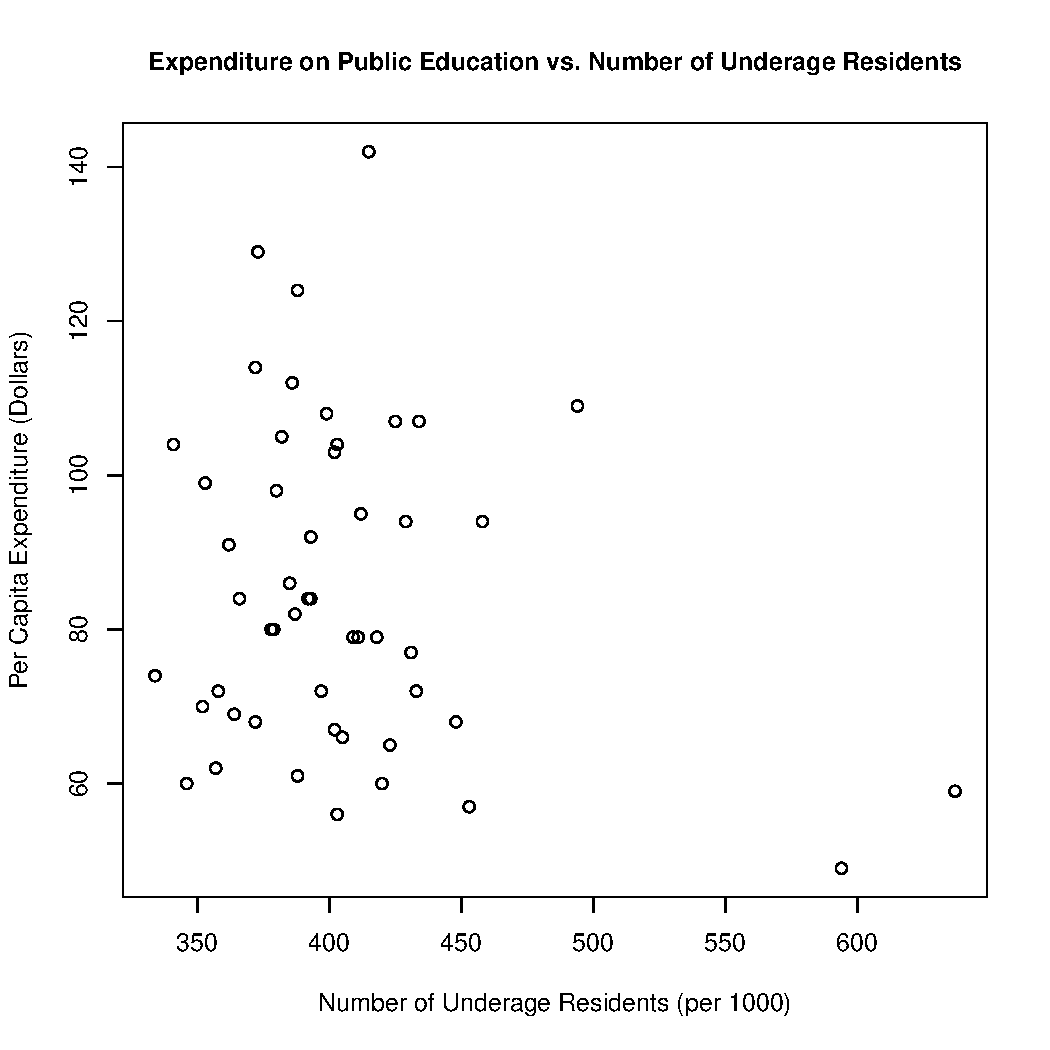
\includegraphics[width=0.7\linewidth]{Graph1}
	\caption{Relationship between Y and X2}
	\label{fig:graph1}
\end{figure}

\noindent The graph shows a weak to no correlation between the number of residents under 18 years old and the per capita expenditure on public education. This is interesting since I expected an increased demand and expenditure for public education with more children/teenagers. 

\vspace{0.5cm}

\noindent Also, there are a few outliers with unusually large numbers of underage residents and corresponding low per capita expenditure on public education.

\newpage
\begin{figure} [h]
	\centering
	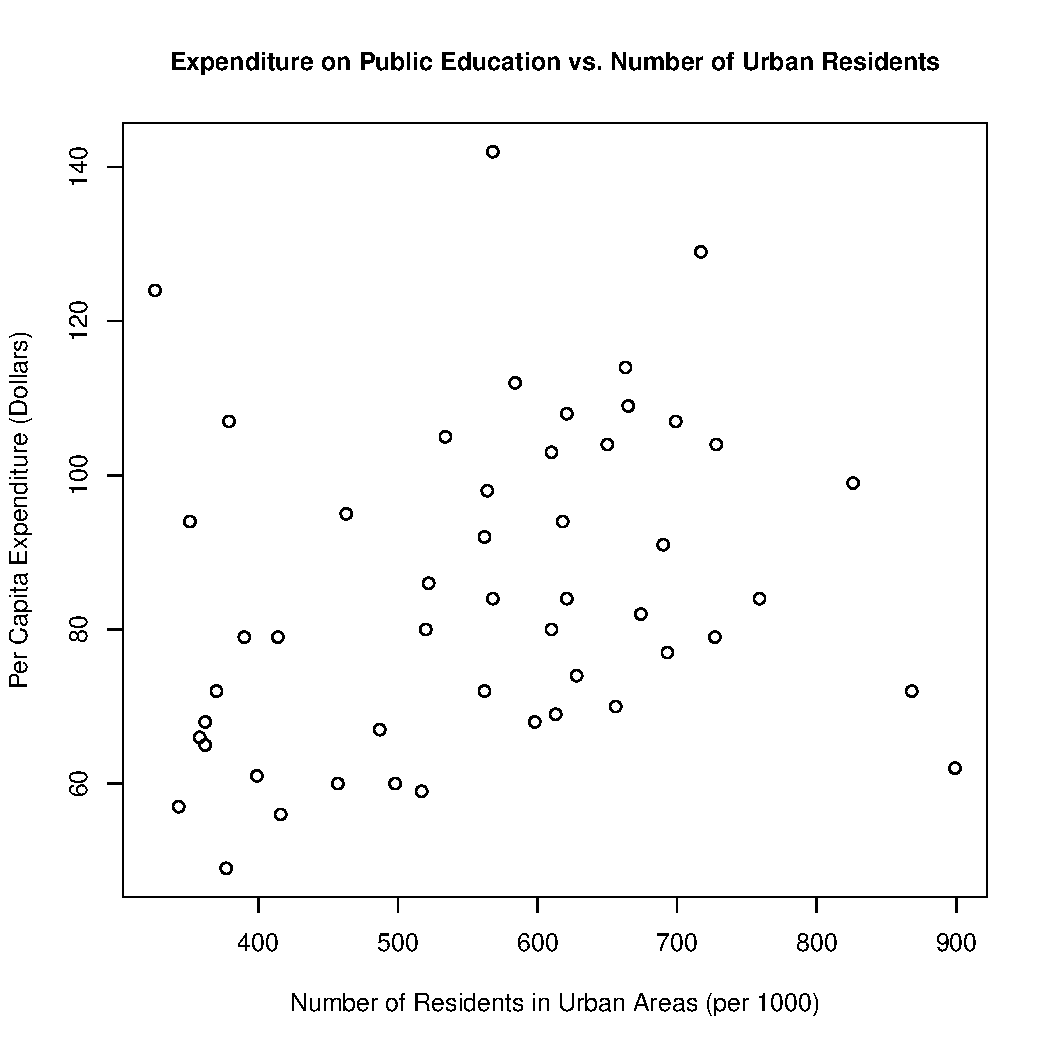
\includegraphics[width=0.7\linewidth]{Graph2}
	\caption{Relationship between Y and X3}
	\label{fig:graph3}
\end{figure}

The graph shows a weak to moderate, positive, linear correlation between the number of residents in urban area and the per capita expenditure on public education. Since population density in urban areas are greater than that of rural areas, the expenditure on public education may be greater as a result.
\newpage 
\begin{figure} [h]
	\centering
	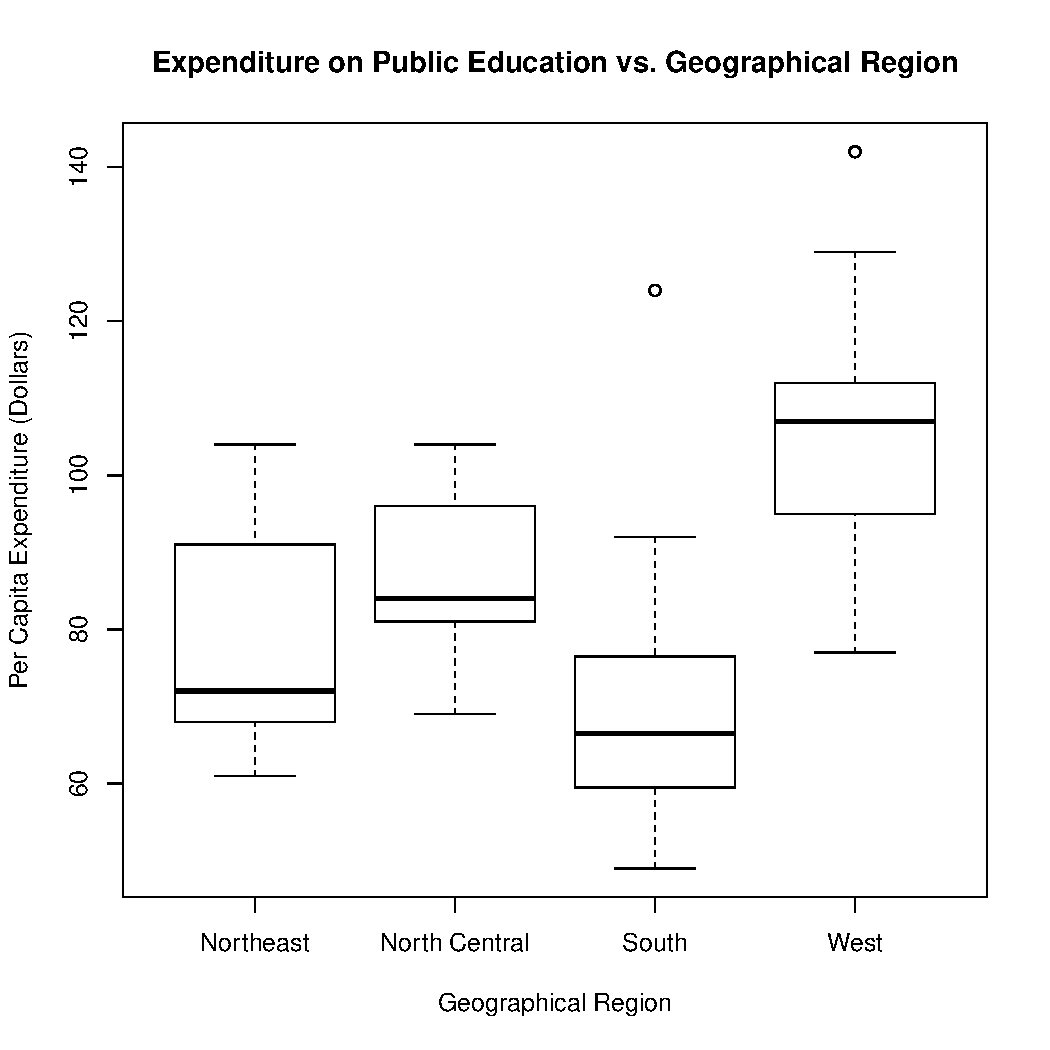
\includegraphics[width=0.7\linewidth]{Graph3}
	\caption{Relationship between Y and Region}
	\label{fig:graph2}
\end{figure}

\noindent First, I recoded the variable Region to show names of the regions instead of numbers.

\lstinputlisting[language=R, firstline=104, lastline=108]{PS1_Answers.R}

\noindent On average, states in the West have the highest per capita expenditure on public education compared to other states. 

\vspace{0.5cm}

\noindent Using the summarySE function also shows that the average expenditure on public education is greatest in the West.

\lstinputlisting[language=R, firstline=109, lastline=109]{PS1_Answers.R}

\begin{figure} [h]
	\centering
	\includegraphics[width=0.6\linewidth]{../../../../../Desktop/data}
	\caption{Result from summarySE}
	\label{fig:data}
\end{figure}

\newpage
\begin{figure} [h]
	\centering
	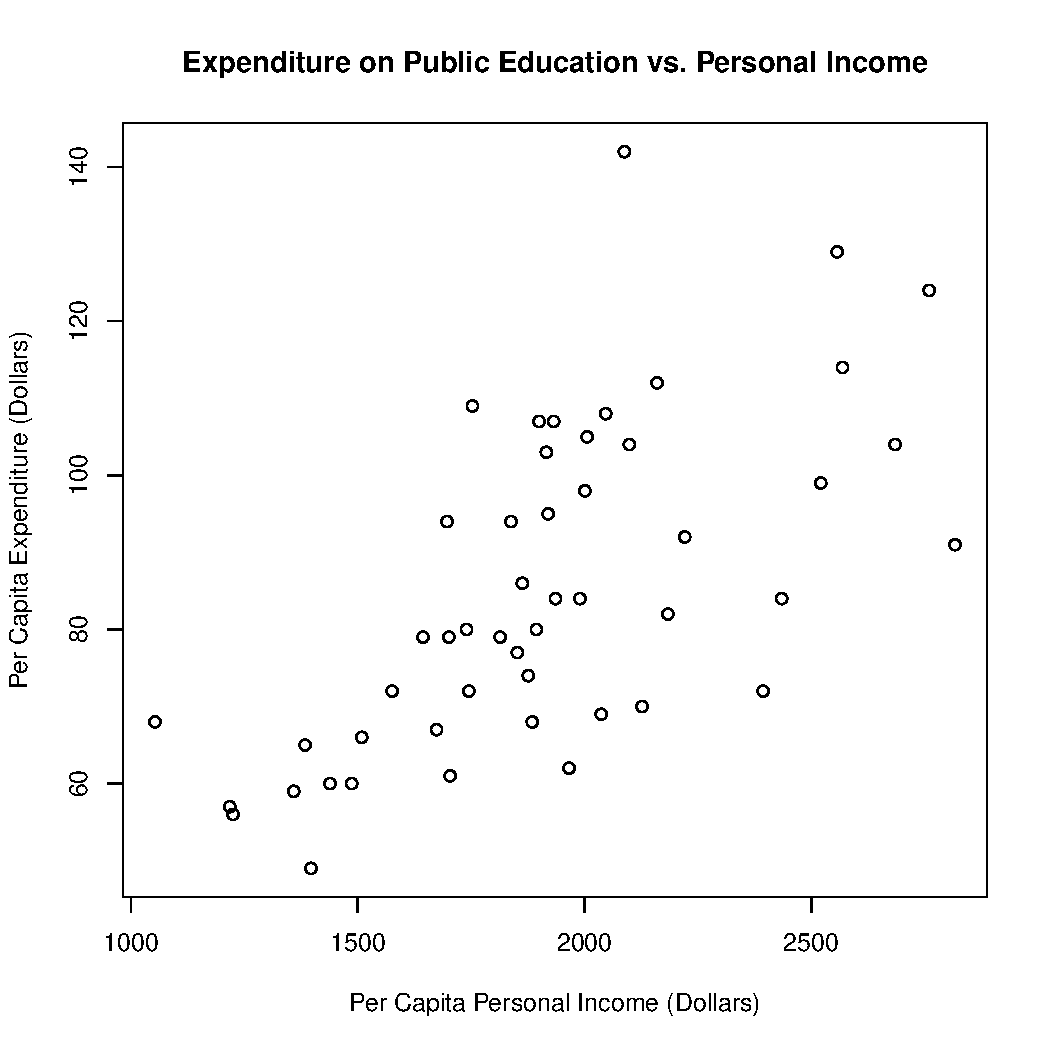
\includegraphics[width=0.7\linewidth]{Graph4}
	\caption{Relationship between Y and X1 }
	\label{fig:graph2}
\end{figure}

\noindent There is a moderate to strong, positive, linear correlation between personal income and per capita expenditure on public education. Since communities with higher income have higher spending power, expenditure on public education may be greater as a result.

\newpage
\begin{figure} [h]
	\centering
	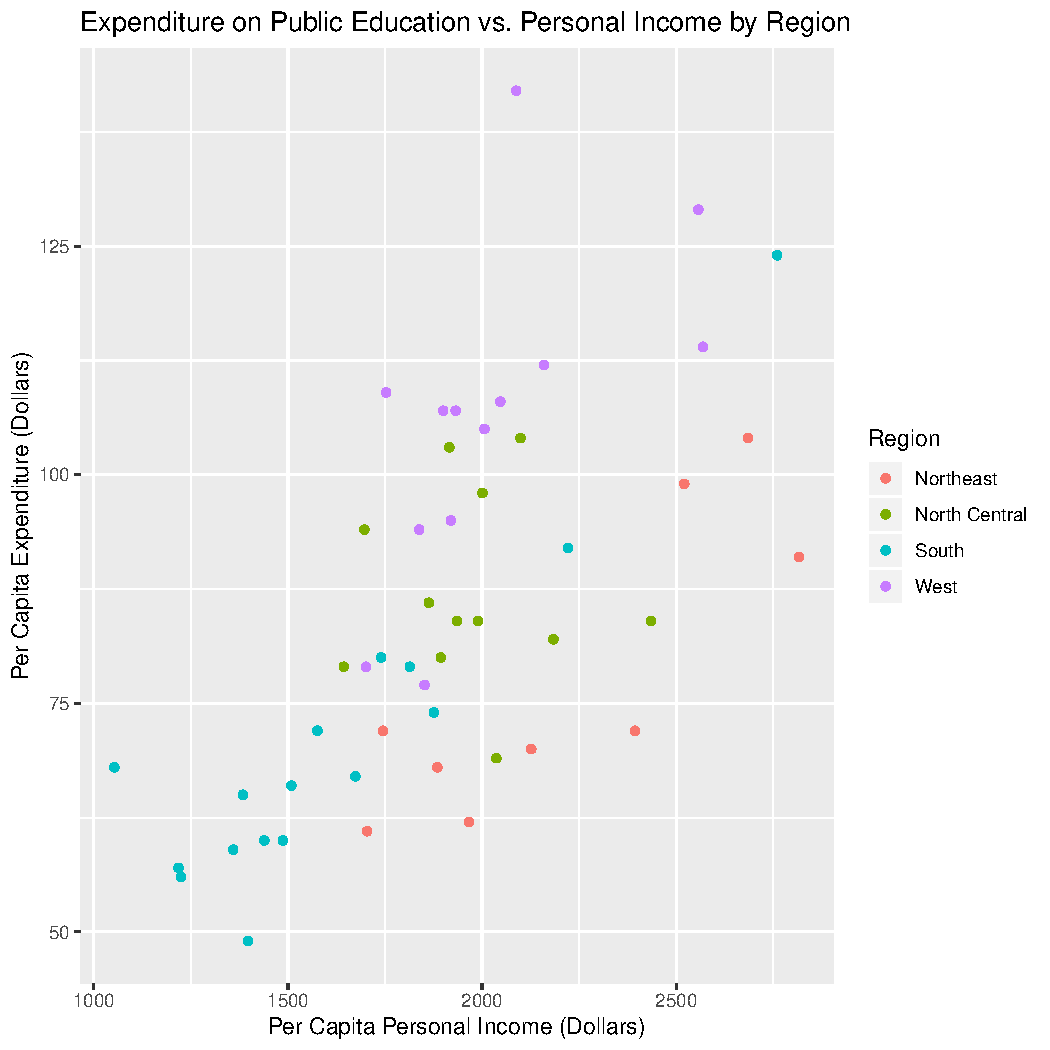
\includegraphics[width=0.9\linewidth]{Graph5}
	\caption{Relationship between Y and X1 illustrated with Respective Regions Colored}
	\label{fig:graph2}
\end{figure}

\noindent Based on this graph, we can see that the Western region tend to have higher expenditure compared to other regions and has moderate to high per capita income. In contrast, the South tends to have lower per capita income and lower per capita expenditure. It would be interesting to explore the infrastructure and the public policy of different regions to see how they interact with variables like individual income and expenditure on public education.

\end{itemize}

\end{document}
